\documentclass{article}
% translate with >> pdflatex -shell-escape <file>

% This file is an extract of the PGFPLOTS manual, copyright by Christian Feuersaenger.
% 
% Feel free to use it as long as you cite the pgfplots manual properly.
%
% See
%   http://pgfplots.sourceforge.net/pgfplots.pdf
% for the complete manual.
%
% Any required input files (for <plot table> or <plot file> or the table package) can be downloaded
% at
% http://www.ctan.org/tex-archive/graphics/pgf/contrib/pgfplots/doc/latex/
% and
% http://www.ctan.org/tex-archive/graphics/pgf/contrib/pgfplots/doc/latex/plotdata/

\usepackage{pgfplots}
\pgfplotsset{compat=newest}

\pagestyle{empty}
\usepgfplotslibrary{dateplot}\usepackage{eurosym}

\begin{document}
% requires \usepgfplotslibrary{dateplot} !
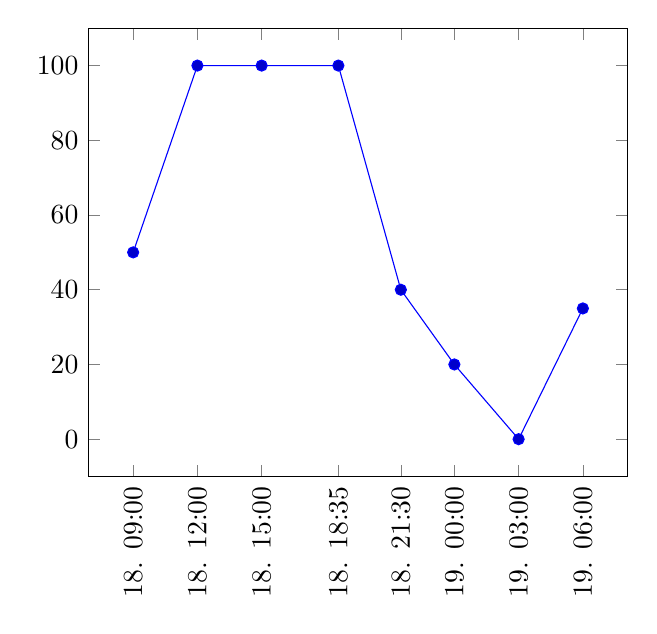
\begin{tikzpicture}
  \begin{axis}[
    date coordinates in=x,
    xtick=data,
    xticklabel style=
		{rotate=90,anchor=near xticklabel},
    xticklabel=\day. \hour:\minute,
    date ZERO=2009-08-18,% <- improves precision!
  ]
  \addplot coordinates {
    (2009-08-18 09:00,  050)
    (2009-08-18 12:00,  100)
    (2009-08-18 15:00,  100)
    (2009-08-18 18:35,  100)
    (2009-08-18 21:30,  040)
    (2009-08-19,        020)
    (2009-08-19 3:00,   000)
    (2009-08-19 6:0,    035)
  };
  \end{axis}
\end{tikzpicture}
\end{document}
